%--------------------------------------------------------------------
% NE 155 (intro to numerical simulation of radiation transport)
% Spring 2014

% formatting
\documentclass[12pt]{article}
\usepackage[top=1in, bottom=1in, left=1in, right=1in]{geometry}

\usepackage{setspace}
\onehalfspacing

\setlength{\parindent}{0mm} \setlength{\parskip}{1em}


% packages
\usepackage{amssymb}
%% The amsthm package provides extended theorem environments
\usepackage{amsthm}
\usepackage{epsfig}
\usepackage{times}
\renewcommand{\ttdefault}{cmtt}
\usepackage{amsmath}
\usepackage{graphicx} % for graphics files

% Draw figures yourself
\usepackage{tikz} 

% The float package HAS to load before hyperref
\usepackage{float} % for psuedocode formatting
\usepackage{xspace}

% from Denovo methods manual
\usepackage{mathrsfs}
\usepackage[mathcal]{euscript}
\usepackage{color}
\usepackage{array}

\usepackage[pdftex]{hyperref}

\newcommand{\nth}{n\ensuremath{^{\text{th}}} }
\newcommand{\ve}[1]{\ensuremath{\mathbf{#1}}}
\newcommand{\macro}{\ensuremath{\Sigma}}
\newcommand{\vOmega}{\ensuremath{\hat{\Omega}}}

\newcommand{\cc}[1]{\ensuremath{\overline{#1}}}
\newcommand{\ccm}[1]{\ensuremath{\overline{\mathbf{#1}}}}


%--------------------------------------------------------------------
%--------------------------------------------------------------------
\begin{document}
\begin{center}
{\bf NE 155, Classes 21-23, S14 \\
Finite Difference Methods for the eigenvalue form of the DE \\ March 17, 2014}
\end{center}

\setlength{\unitlength}{1in}
\begin{picture}(6,.1) 
\put(0,0) {\line(1,0){6.25}}         
\end{picture}

%--------------------------------------------------------------------
\section{Finite Difference Method, Eigenvalue Problem}

We can extend all of the things that we just did to the eigenvalue problem case, which is another layer of complication. 

Now instead of a fixed source, we have an eigenvalue problem
\[-\frac{d}{dx}D(x)\frac{d \phi(x)}{dx} + \Sigma_a(x) \phi(x) = \frac{1}{k}\nu \Sigma_f(x) \phi(x) \]
%
\begin{figure}[h!]
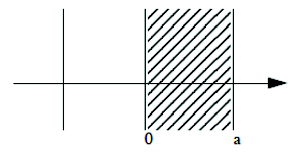
\includegraphics[height=1in]{FVM-fig}
\end{figure}
%
Let's again have a reflecting condition at the centerline ($x_0 = 0$) and vacuum on the right ($x_n = a$):
\begin{align}
\frac{d}{dx}\phi(x) \big|_{x=0} &= 0 \qquad \text{zero net current} \nonumber\\
\phi(\tilde{a}) &= 0 \qquad \tilde{a} = a + 2D \nonumber
\end{align}

We again have a spatial mesh:
%
\begin{center}
\begin{tikzpicture}
\draw (-.25,0)--(1.25,0);
\draw[dotted] (1.25,0)--(2.75,0);
\draw (2.75,0)--(5.25,0);
\draw[dotted] (5.25,0)--(6.75,0);
\draw (6.75,0)--(8.25,0);
%\draw (4,0)--(5.25,0);
\draw (0,-.25)--(0,.25);
\draw (1,-.25)--(1,.25);
%\draw (2,-.25)--(2,.25);
\draw (3,-.25)--(3,.25);
\draw (4,-.25)--(4,.25);
\draw (5,-.25)--(5,.25);
\draw (7,-.25)--(7,.25);
\draw (8,-.25)--(8,.25);
\node[below] at (0,-.25) {$x_0 = 0$};
\node[below] at (1,-.25) {$x_1$};
\node[below] at (3,-.25) {$x_{i-1}$};
\node[below] at (4,-.25) {$x_i$};
\node[below] at (5,-.25) {$x_{i+1}$};
\node[below] at (7,-.25) {$x_{n-1}$};
\node[below] at (8,-.25) {$x_n = a$};
\node[above] at (0.5, 0.5) {$h_1$};
\node[above] at (3.5, 0.5) {$h_i$};
\end{tikzpicture}
\end{center}
%
and in this configuration $x_0 = 0$, $x_n = a$, and $h$ is the mesh spacing. There are $n+1$ points and $n$ mesh cells.

Material discontinuities will coincide with the cell edges, $x_i$. Thus, we can assume that the cross sections and the diffusion coefficient are constant in each cell:
%
\begin{align}
D(x) &= D_i \qquad \text{for } x_{i-1} \leq x_i \nonumber \\
\Sigma_{a}(x) &= \Sigma_{a,i} \qquad \text{for } x_{i-1} \leq x_i \nonumber \\
\nu\Sigma_f(x) &= \nu\Sigma_{f,i}\;, \qquad \text{for } x_{i-1} \leq x \leq x_i \nonumber \\
h_i &\equiv x_i - x_{i-1} \nonumber 
\end{align}
%
The unknown fluxes and known sources are again defined at the mesh or cell edges:
\begin{align}
\phi(x_i) &= \phi_i \nonumber \\
S(x_i) &= S_i \nonumber 
\end{align}
%
With this formulation we still have the problem that our unknown is defined the cell edges and if the properties in neighboring cells differ we will have discontinuities. To be able to handle \textit{material discontinuities} we're going to do our volume integration again.


%-----------------------------------------------------
%-----------------------------------------------------
\section{Finite Volume Method}

Like last time, we will integrate the flux and source values across neighboring half-cells.
%
\begin{figure}[h!]
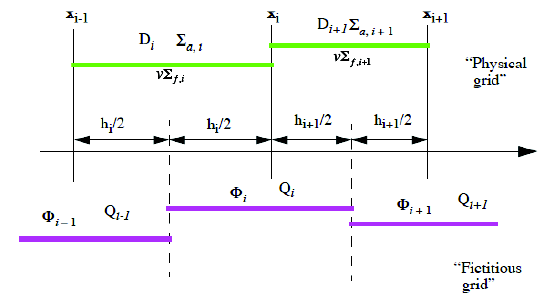
\includegraphics[height=2.5in]{FVM-eig-fig}
\end{figure}

We again assume the cross section and diffusion coefficient are constant in each cell 
\begin{align}
D(x) &= D_i\;, \qquad x_{i-1} \leq x \leq x_i \nonumber \\
\Sigma_a(x) &= \Sigma_{a,i}\;, \qquad x_{i-1} \leq x \leq x_i \nonumber \\
\nu\Sigma_f(x) &= \nu\Sigma_{f,i}\;, \qquad x_{i-1} \leq x \leq x_i \nonumber \\
h_i &\equiv x_{i} - x_{i-1} \nonumber 
\end{align}
%
We further assume that the fluxes and sources are constant over the interval centered around $x_i$:
%
\begin{align}
\phi(x) &= \phi_i \qquad \text{for } \bigl(x_i - \frac{h_i}{2}\bigr) \leq x \leq \bigl(x_i + \frac{h_{i+1}}{2}\bigr) \nonumber \\
S(x) &= S_i \qquad \text{for } \bigl(x_i - \frac{h_i}{2}\bigr) \leq x \leq \bigl(x_i + \frac{h_{i+1}}{2}\bigr) \nonumber 
\end{align}

Now, we integrate the differential equation over each cell, $\bigl(x_i - \frac{h_i}{2}\bigr) \leq x \leq \bigl(x_i + \frac{h_{i+1}}{2}\bigr)$:
%
\[\int_{(x_i - \frac{h_i}{2})}^{(x_i + \frac{h_{i+1}}{2})} \biggl(  -\frac{d}{dx}D(x)\frac{d \phi(x)}{dx}\biggr) dx 
+ \int_{(x_i - \frac{h_i}{2})}^{(x_i + \frac{h_{i+1}}{2})} \Sigma_a(x) \phi(x) dx 
= \int_{(x_i - \frac{h_i}{2})}^{(x_i + \frac{h_{i+1}}{2})} \frac{1}{k}\nu \Sigma_f(x) \phi(x) dx\]
%
We'll only add the term we didn't do before:
%
\begin{align}
\int_{(x_i - \frac{h_i}{2})}^{(x_i + \frac{h_{i+1}}{2})} \frac{1}{k}\nu \Sigma_f(x) \phi(x) \phi(x) dx &= 
%
\int_{(x_i - \frac{h_i}{2})}^{(x_i)} \frac{1}{k}\nu \Sigma_f(x) \phi(x) dx + \int_{(x_i)}^{(x_i + \frac{h_{i+1}}{2})} \frac{1}{k}\nu \Sigma_f(x) \phi(x) dx \nonumber\\&=
%
\frac{1}{k} \biggl(\frac{\nu\Sigma_{f,i}h_i + \nu\Sigma_{f,i+1}h_{i+1}}{2} \biggr)\phi_i \nonumber 
\end{align}

Collecting all of the terms:
%
\begin{equation}
-D_{i+1}\biggl(\frac{\phi_{i+1} - \phi_i}{h_{i+1}}\biggr) + D_{i}\biggl(\frac{\phi_{i} - \phi_{i-1}}{h_{i}}\biggr) + \biggl(\frac{\Sigma_{a,i}h_i + \Sigma_{a,i+1}h_{i+1}}{2} \biggr)\phi_i =   \frac{1}{k} \biggl(\frac{\nu\Sigma_{f,i}h_i + \nu\Sigma_{f,i+1}h_{i+1}}{2} \biggr)\phi_i \nonumber
\end{equation}

To express this in matrix form we'll use some abbreviations as last time, and add one for the fission term (where we've divided through by $h_{ii}$ to get the x-sec terms):
\begin{align}
h_{ii} &= \frac{h_i + h_{i+1}}{2} \nonumber \\
%
\Sigma_{a,ii} &= \frac{\Sigma_{a,i}h_i + \Sigma_{a,i+1}h_{i+1}}{h_i + h_{i+1}} \nonumber \\
\nu\Sigma_{f,ii} &= \frac{\nu\Sigma_{f,i}h_i + \nu\Sigma_{f,i+1}h_{i+1}}{h_i + h_{i+1}} \nonumber
\end{align}
%
Then
%
\[a_{i,i-1} \phi_{i-1} + a_{i,i}\phi_i + a_{i, i+1} \phi_{i+1} = \frac{1}{k}\nu\Sigma_{f,ii} \phi_i \qquad \text{for } i = 1, 2, \dots, n-1\]
%
where the $a$s have the same value as last time. 
%
\begin{align}
a_{i,i-1} &= \frac{-D_i}{h_i h_{ii}} \nonumber \\
a_{i,i} &= \frac{D_i}{h_i h_{ii}} + \frac{D_{i+1}}{h_{i+1} h_{ii}} +\Sigma_{a,ii} \nonumber \\
a_{i,i+1} &= \frac{-D_{i+1}}{h_{i+1} h_{ii}} \nonumber
\end{align}

And again we have a set of $n-1$ linear algebraic equations with $n+1$ unknowns. We will use the boundary conditions to get the rest of the information that we need.


%-------------------------------------------------------
\subsection{Boundary Conditions}

Again assume $x_n = \tilde{a}$, then the \textbf{vacuum condition} becomes
\[\phi_n = 0\]
and the last equation for $i=n-1$ becomes
\[a_{n-1,n-2} \phi_{n-2} + a_{n-1,n-1}\phi_{n-1} + 0 = \frac{1}{k}\nu\Sigma_{f,ii} \phi_{n-1}\]

To include the \textbf{reflecting} or zero current condition we integrate over $[0, h_{1}/2]$.
%
\begin{figure}[h!]
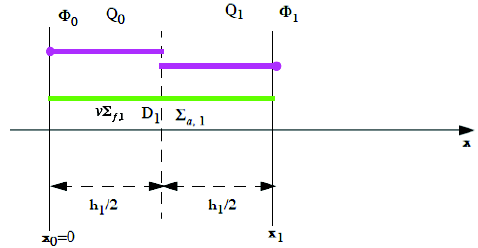
\includegraphics[height=2in]{ReflectingBC-eig}
\end{figure}
%
\begin{align}
\int_{0}^{\frac{h_{1}}{2}} \biggl(-\frac{d}{dx}D(x)\frac{d \phi(x)}{dx}\biggr) dx &+ \int_{0}^{\frac{h_{1}}{2}} \Sigma_a(x) \phi(x) dx = \int_{0}^{\frac{h_{1}}{2}} \frac{1}{k}\nu \Sigma_f(x) \phi(x) dx \nonumber \\
%
-D(x)\frac{d \phi(x)}{dx}\big|_{\frac{h_{1}}{2}} &+ D(x)\frac{d \phi(x)}{dx}\big|_{0} + \Sigma_{a,1}\phi_0 \frac{h_1}{2} = \frac{1}{k}\nu\Sigma_{f,1} \phi_0 \frac{h_1}{2} \nonumber 
\end{align}
%
Now we can apply the boundary condition $\frac{d \phi(x)}{dx}\big|_{0} = 0$ to get:
\[-D(x)\frac{d \phi(x)}{dx}\big|_{\frac{h_{1}}{2}} + \Sigma_{a,1}\phi_0 \frac{h_1}{2} = \frac{1}{k}\nu\Sigma_{f,1} \phi_0 \frac{h_1}{2}\]
%
Recall that
\[-D(x)\frac{d \phi(x)}{dx}\big|_{\frac{h_{1}}{2}} \cong -D_{1}\biggl(\frac{\phi_{1} - \phi_0}{h_{1}}\biggr) \]

And the first equation ($i=0$) becomes
\[a_{00}^*\phi_0 + a_{01}^* \phi_1 = \frac{1}{k}\nu\Sigma_{f,1} \phi_0 \:,\]
%
where we redefine the $a$s to be (I've added the * to indicate that these have different definitions than the rest of the terms.)
%
\begin{align}
a_{00}^* &= \frac{2D_1}{h_1^2} + \Sigma_{a,1} \nonumber \\
a_{01}^* &= -\frac{2D_1}{h_1^2} \nonumber 
\end{align}

We now have $n$ equations and $n$ unknowns, but we formulate it a bit differently: 
\[\ve{A}\vec{\phi} = \frac{1}{k}\ve{F}\vec{\phi}\]
where:
\begin{align}
\ve{A} &= \begin{pmatrix}
a_{00}^* & a_{01}^* & 0      & 0 & \cdots & 0 \\
a_{10}   & a_{11}   & a_{12} & 0 & \cdots & 0 \\
0        & a_{21}   & a_{22}   & a_{21} &  & \vdots \\
\vdots        &    & \ddots  & \ddots & \ddots & \vdots \\
0 & \cdots & 0 & a_{n-3,n-3}   & a_{n-2,n-2} & a_{n-2,n-1} \\
0        & \cdots   & 0   & 0 & a_{n-1,n-2} & a_{n-1,n-1} 
\end{pmatrix} \nonumber \\
%
\vec{\phi} &= \begin{pmatrix}\phi_0 \\ \phi_1 \\ \phi_2 \\ \vdots \\ \phi_{n-2} \\ \phi_{n-1} \end{pmatrix} \:, \qquad
%
\ve{F} = \begin{pmatrix}
\nu\Sigma_{f,11} & 0 & 0 & \cdots & 0 \\
0   & \nu\Sigma_{f,22}   & 0 & \cdots & 0 \\
\vdots        & \ddots  & \ddots & \ddots & \vdots \\
0 & \cdots & 0 & \nu\Sigma_{f,n-1,n-1} & 0 \\
0        & \cdots   & 0   & 0 & \nu\Sigma_{f,nn} 
\end{pmatrix} \nonumber
\end{align}

%----------------------------------------------------------------
\subsection{Homogeneous, Uniform Mesh}

If we end up having a homogeneous system with a uniform mesh, then we can make some simplifications.
%
\begin{align}
&h_i = h \nonumber \\
&D_i = D \nonumber \\
&\Sigma_{a,i} = \Sigma_a \nonumber \\
%
&\frac{-D}{h^2}\phi_{i-1} + \biggl(\frac{2D}{h^2} + \Sigma_a \biggr)\phi_i - \frac{D}{h^2}\phi_{i+1} = S_i \qquad \text{for } i = 1, \dots, n-2 \nonumber \\
%
&\biggl(\frac{2D}{h^2} + \Sigma_a \biggr) \phi_0 - \frac{D}{h^2}\phi_{1} = S_0 \qquad \text{for } i = 0 \nonumber \\
%
&\frac{-D}{h^2}\phi_{n-2} + \biggl(\frac{2D}{h^2} + \Sigma_a \biggr)\phi_{n-1} = S_{n-1} \qquad \text{for } i = n-1 \nonumber
\end{align}


%----------------------------------------------------------------
%----------------------------------------------------------------
\section{Solution Methods}

Both the FDM and FVM result in tridiagonal systems. Recall that formally solving these systems looks like
\[\vec{\phi} = \ve{A}^{-1}\vec{S} \:.\]
There are a few ways that we can solve these. 

%----------------------------------------------------------------
\subsection{Directly}

Tridiagonal systems can be solved directly using Gaussian elimination. 

This is not a bad option in our case because $\ve{A}$ is diagonally dominant (each diagonal element is greater than the sums of the absolute values of the off-diagonal elements in the same row):
\[a_{ii} \geq |a_{i,i-1}| + |a_{i, i+1}|\:.\] 

The general algorithm to solve a tridiagonal system is short and easy, it's called the \textbf{Thomas Algorithm}. We covered it back with general linear solution methods. 

%How do we develop an algorithm to execute this that can be easily programmed? 
\underline{Would you like to go through that a little more slowly or move to the next thing?}

Let's start by writing our system this way:
%
\begin{equation}
\begin{pmatrix}
B_0  & -C_0 & 0    & 0    & \cdots & 0 \\
-A_1 & B_1  & -C_1 & 0    & \cdots & 0 \\
0    & -A_2 & B_2  & -C_2 & & \vdots \\
\vdots        &    & \ddots  & \ddots & \ddots & \vdots \\
0 & \cdots & 0 & -A_{n-2} & B_{n-2} & -C_{n-2} \\
0        & \cdots   & 0   & 0 & -A_{n-1} & B_{n-1} 
\end{pmatrix}
%
\begin{pmatrix}\phi_0 \\ \phi_1 \\ \phi_2 \\ \vdots \\ \phi_{n-2} \\ \phi_{n-1} \end{pmatrix} =
%
\begin{pmatrix}S_0 \\ S_1 \\ S_2 \\ \vdots \\ S_{n-2} \\ S_{n-1} \end{pmatrix}
\end{equation}
%
Recall that $\phi_n = 0$. 

To develop the algorithm, let's look at a 3$\times$3 system of equations.
\begin{align}
B_0\phi_0 - C_0\phi_1 \hspace*{3.25em}&= S_0 \nonumber \\
-A_1\phi_0 + B_1\phi_1 - C_1\phi_3 &= S_1 \nonumber \\
-A_2\phi_1 + B_2\phi_2 &= S_2 \nonumber 
\end{align}
%
Now the process:
\begin{enumerate}
\item Define
\[u_0 = B_0 \qquad v_0 = S_0\]
and write the first equation as
\[u_0\phi_0 - C_0\phi_1 = v_0\]

\item multiply by $A_1 / u_0$
\[A_1\phi_0 - \frac{A_1 C_0}{u_0}\phi_1 = \frac{A_1 v_0}{u_0}\]
Now add this to the second equation (where the $\phi_0$ term subtracts out)
\[\biggl(B_1-\frac{A_1 C_0}{u_0}\biggr)\phi_1 - C_1\phi_3 = S_1 + \frac{A_1 v_0}{u_0}\]
%
and define
\[u_1 = B_1-\frac{A_1 C_0}{u_0} \qquad v_1 = S_1 + \frac{A_1 v_0}{u_0}\]
to re-write as
\[u_1\phi_1 - C_1\phi_2 = v_1\:.\]

\item Guess what's next? Multiply this equation by $A_2 / u_1$
\[A_2\phi_1 - \frac{A_2 C_1}{u_1}\phi_2 = \frac{A_2 v_1}{u_1}\]
and add to the third equation
\[\biggl(B_2-\frac{A_2 C_1}{u_1}\biggr)\phi_2 = S_2 + \frac{A_2 v_1}{u_1}\]
%
and define
\[u_2 = B_2-\frac{A_2 C_1}{u_1} \qquad v_2 = S_2 + \frac{A_2 v_1}{u_1}\]
to re-write as
\[u_2\phi_2 = v_2 \:.\]
\end{enumerate}
%
All together we now have an \textbf{upper triangular system}:
\begin{align}
u_0\phi_0 - C_0\phi_1 \hspace*{3.25em} &= v_0 \nonumber \\
u_1\phi_1 - C_1\phi_2 &= v_1 \nonumber \\
u_2\phi_2 &= v_2 \nonumber
\end{align}
%
that we can solve with \textbf{backward substitution}.

Here's the compact form of the algorithm (the Thomas algorithm)
\begin{enumerate}
\item \[u_0 = B_0 \qquad v_0 = S_0\]

\item for $i=1, \dots, n-1$
\[u_i = B_i-\frac{A_i C_{i-1}}{u_{i-1}} \qquad v_i = S_i + \frac{A_i v_{i-1}}{u_{i-1}}\]

\item Backward sub starting with $i=n-1$
\[\phi_{n-1} = \frac{v_{n-1}}{u_{n-1}}\]

\item Then for $i= n-2, \dots, 1$
\[\phi_i = \frac{1}{u_i}\bigl(v_i + C_i \phi_{i+1}\bigr)\]
\end{enumerate}

That was pretty easy,but we typically try to \textit{avoid direct inversion of matrices} because it might be expensive in time and/or memory, round-off error, instability, etc.

We often use an iterative method instead. 


%----------------------------------------------------------------
\subsection{Iterative Methods}

Recall: produce a sequence of vectors, $\vec{\phi}^{(1)}, \vec{\phi}^{(2)}, \dots$ based on the prescription
  \[\vec{\phi}^{(k+1)} = F(\vec{\phi}^{(k)}, \vec{S})\:, \qquad \text{where } \displaystyle \lim_{k \rightarrow \infty} \vec{\phi}^{(k)} = \vec{\phi}\] 
%
\begin{align}
(\ve{A} + \ve{B}) \vec{\phi} &= \ve{B}\vec{x} + \vec{S} \nonumber \\
%
\ve{C} \vec{\phi} &= \ve{B}\vec{\phi} + \vec{S} 
\qquad\text{where } \ve{C} = \ve{A} + \ve{B} \nonumber \\
%
\vec{\phi} &= \ve{C}^{-1} \ve{B}\vec{\phi} + \ve{C}^{-1} \vec{S} 
\nonumber \\
%
\vec{\phi} &= \ve{P}\vec{\phi} + \tilde{\vec{S}}  
\qquad\text{assuming regular } \ve{C}\nonumber
\end{align}
%
And the \textbf{fixed-point} iterative process is:
\begin{align}
\vec{\phi}^{(0)} &= \text{ arbitrary}\nonumber \\
\vec{\phi}^{(k+1)} &= \ve{P}\vec{\phi}^{(k)} + \tilde{\vec{S}} \nonumber
\end{align}

How we split $\ve{A}$ determines what method we're doing.

\subsubsection{Jacobi}

Let $\ve{D} = diag(\ve{A})$, then
\begin{align}
\ve{D} \vec{\phi}^{k+1} &= (\ve{D} - \ve{A})\vec{\phi}^{(k)} + \vec{S} \nonumber \\
%
\vec{\phi}^{k+1} &= \ve{D}^{-1}(\ve{D} - \ve{A})\vec{\phi}^{(k)} + \ve{D}^{-1}\vec{S} \nonumber
\end{align}
%
In our original syntax, $\ve{P}_J = \ve{I} -  \ve{D}^{-1}\ve{A}$ and $\tilde{\vec{S}} =\ve{D}^{-1}\vec{S}$.

The algorithm for this method is, for $i = 1, \dots, n$:
\[ \phi^{(k+1)}_i = \frac{1}{a_{ii}}(S_i - \sum_{j=1}^{i-1} a_{ij} \phi_j^{(k)} - \sum_{j=i+1}^{n} a_{ij} \phi_j^{(k)})\]

We can apply Gauss Seidel and SOR in exactly the same way. 




%--------------------------------------------------------------------
%--------------------------------------------------------------------
%\bibliographystyle{plain}
%\bibliography{LinearSolns} 

\end{document}